\documentclass[a4paper]{report}

% Incluir los paquetes necesarios
\usepackage[utf8]{inputenc}
\usepackage[spanish]{babel}
\usepackage[bookmarks=false,colorlinks=true,linkcolor={blue},pdfstartview={XYZ null null 1.22}]{hyperref}
\usepackage[pdftex]{graphicx}
\usepackage[style=list]{glossary}
\usepackage{fancyhdr}
\usepackage{epigraph} %para los quote en cada capitulo
\usepackage[usenames,dvipsnames]{color}
\usepackage{listings}
\usepackage{caption}

% \pagestyle{fancy}
% \fancyfoot{}

% \fancyhead[CO,CE]{---Draft---}
% \fancyfoot[CO,CE]{Confidential}
% \fancyfoot[RO, LE] {\thepage}
%\renewcommand{\headrulewidth}{0.4pt}
% \renewcommand{\footrulewidth}{0.4pt}

% Título, autor(es), fecha.
\title{Sistemas Web Desconectados}
\author{Defossé Nahuel, van Haaster Diego Marcos}
\date{\today}

\pagestyle{fancy}
%\fancyhead{}
\renewcommand\headrulewidth{.1pt}
%\fancyhead[LO,RE]{\footnotesize\sffamily\lite\leftmark}
%\fancyhead[LE,RO]{\footnotesize\sffamily\lite\itshape\rightmark}
% Esta fuente es muy grande y se pisan los titulos
%\fancyhead[LO,RE]{\footnotesize\lite\leftmark}
%\fancyhead[LE,RO]{\footnotesize\lite\itshape\rightmark}
\fancyfoot[c]{\thepage}
%\fancyfoot[LE,RO]{\setlength{\fboxsep}{2pt}\ovalbox{\footnotesize\sffamily\thepage}}
%\fancyfoot[LO,RE]{\footnotesize\sffamily\lite\@title}
%\fancyfoot[R]{\setlength{\fboxsep}{2pt}{\ovalbox{\footnotesize\sffamily\thepage}}}
%\fancyfoot[L]{\footnotesize\sffamily\lite\thepage}

%Comandos
\newcommand{\fullref}[1]{\ref{#1} de la página \pageref{#1}}

%Crear el glosario
\makeglossary

%Colores
\definecolor{gray97}{gray}{.97}
\definecolor{gray80}{gray}{.80}
\definecolor{gray45}{gray}{.45}

%Formato de los bloques con codigo fuente
\lstset{
    frame=Ltb,
    framerule=0pt,
    aboveskip=0.5cm,
    framextopmargin=3pt,
    framexbottommargin=3pt,
    framexleftmargin=0.4cm,
    framesep=0pt,
    rulesep=.4pt,
    backgroundcolor=\color{gray97},
    rulesepcolor=\color{black},
    %
    stringstyle=\color{ForestGreen}\ttfamily,
    showstringspaces = false,
    basicstyle=\small\ttfamily,
    commentstyle=\color{gray45},
    keywordstyle=\color{RedOrange}\bfseries,
    %
    numbers=left,
    numbersep=15pt,
    numberstyle=\tiny,
    numberfirstline = false,
    breaklines=true,                % sets automatic line breaking
    breakatwhitespace=false,        % sets if automatic breaks should only happen at whitespace
    escapeinside={\%*}{*)}          % if you want to add a comment within your code
}

\lstdefinestyle{consola}{
  basicstyle=\scriptsize\bf\ttfamily,
  backgroundcolor=\color{gray80},
  numbers=none,
  framexleftmargin=0pt,
  framexrightmargin=6pt,
  keywordstyle=\color{NavyBlue}\bfseries,
  otherkeywords={>>>}
}
\lstdefinestyle{python}{
  language=Python
}
\lstdefinestyle{javascript}{
  language=Java,
  otherkeywords={function,var,\$,\$\$}
}

%Formato de los titulos en el codigo
\DeclareCaptionFont{white}{\color{white}}
\DeclareCaptionFormat{listing}{\colorbox{gray45}{\parbox{\textwidth}{#1#2#3}}}
\captionsetup[lstlisting]{format=listing,labelfont=white,textfont=white}

\begin{document}

\maketitle

\pagenumbering{roman}
\tableofcontents
\listoffigures
\listoftables

\chapter*{Agradecimientos}
A nuestros familiares
% A Adrian Holovaty, Simon Willison, Jacob Kaplan-Moss y Wilson Miner por haber desarrollado
% un excelente framework simple y así mismo muy podroso para nuestro lenguaje preferido.
% 
% A Michael Trier por su mantenernos actualizados sobre lo que ocurre en la comunidad con
% su \emph{podcast} \textbf{This Week in Django}
%\begin{abstract}

%\end{abstract}

\pagenumbering{arabic}

%Capitulo introductorio
\chapter{Introducción}
\label{ch:intro}
\epigraph{Yo sólo puedo mostrarte la puerta. Tú eres quien debe atravesarla.}{Morfeo}

\section{Motivación}
Hoy más que ayer, pero seguremente menos que mañana, Internet es ``la red de
redes''. El alto contenido de información 
Hoy en día Internet supone más que un medio para obtener información,
su constante expanción a convetido a esta red en un terreno muy atractivo para
la implementación de sistemas de información.

Las aplicaciones web son populares debido a lo práctico que resulta el navegador
web como cliente de acceso a las mismas.
También resulta fácil actualizar y mantener aplicaciones web sin distribuir e
instalar software a miles de usuarios potenciales.
En la actualidad, existe una gran oferta de frameworks web para facilitar el
desarrollo de aplicaciones web.
Una ventaja significativa de las aplicaciones web es que funcionan
independientemente de la versión del sistema operativo instalado en el cliente.
En vez de crear clientes para los múltiples sistemas operativos, la aplicación
web se escribe una vez y se ejecuta igual en todas partes.
Las aplicaciones web tienen ciertas limitaciones en las funcionalidades que
ofrecen al usuario.
Hay funcionalidades comunes en las aplicaciones de escritorio, como dibujar en
la pantalla o arrastrar y soltar, que no están soportadas por las tecnologías
web estándar.
Los desarrolladores web, generalmente, utilizan lenguajes interpretados o script
en el lado del cliente para añadir más funcionalidades, especialmente para
ofrecer una experiencia interactiva que no requiera recargar la página cada
vez.Recientemente se han desarrollado tecnologías para coordinar estos lenguajes
con tecnologías en el lado del servidor.
Los sistemas operativos actuales de propósito general cuentan con un navegador
web, con posibilidades de acceso a bases de datos y almacenamiento de código y
recursos.
La web, en el ámbito del software, es un medio singular por su ubicuidad y sus
estándares abiertos. El conjunto de normas que rigen la forma en que se generan
y transmiten los documentos a través de la web son regulados por la W3C
(Consorcio World Wide Web). La mayor parte de la web está soportada sobre
sistemas operativos y software de servidor que se rigen bajo licencias
OpenSource1 (Apache, BIND, Linux, OpenBSD, FreeBSD). Los lenguajes con los que
son desarrolladas las aplicaciones web son generalmente OpenSource, como e PHP,
Python, Ruby, Perl y Java. Los frameworks web escritos sobre estos lenguajes
utilizan alguna licencia OpenSource para su distribución; incluso frameworks
basados en lenguajes propietarios son liberados bajo licencias OpenSource.
\section{Objetivos}
Podemos decir que las aplicaciones tradicionales, que no hacen uso de la web,
son más robustas ya que no dependen de una conexión.
Por lo tanto, sería deseable poder dotar a las aplicaciones web de la capacidad
de trabajar cuando no cuentan con conexión.
Si bien los elementos necesarios para llevar a cabo esta tarea están disponibles
actualmente, no están contemplados en los diseños de los frameworks web.
Es decir, cuando una determinada aplicación web debe ser transportada al
cliente, es necesario escribir el código de soporte específico para esa
aplicación.
Un framework no constituye un producto per sé, sino una plataforma sobre la cual
construir aplicaciones.
Consideramos que sería beneficioso aportar una extensión a un framework web
OpenSource que brinde facilidades para transportar las aplicaciones web, basadas
en éste, al cliente de manera que la aplicación que haga uso de nuestra
extensión pueda ser ejecutada a posteriori en el navegador en el cual ha sido
descargada.
El framework web será elegido tras un estudio de las características que
consideramos más importantes para el desarrollo veloz, como la calidad del
mapeador de objetos (entre las características más importantes de éste
buscaremos eficiencia en las consultas a la base de datos, ejecución demorada
para encadenamiento de consultas, implementación de herencia, baja carga de
configuración), la simplicidad para enlazar url's a funciones controladoras,
extensibilidad del sistema de escritura de plantillas. Buscaremos frameworks que
permitan la ejecución transversal de cierto tipo de funciones, para ejecutar
tareas como compresión de salida, sustitución de patrones de texto, caché,
control de acceso, etc.

La World Wide Web, o \emph{web}, durante los últimos años ha ganado terreno como
plataforma para aplicaciones del variado tipo. 
Diversas tecnologías fueron formuladas para convertir el escenario inical, donde
la web se limitaba a ser una gran colección de documentos enlazados
(\emph{hipertexto}),
para llegar a ser...

Vamos a realizar un breve análisis sobre las tecnologías que son utilizadas en
la web.

Luego un análisis de las tecnologías del cliente, haciendo hincapié en ...

http://es.wikiquote.org/wiki/The\_Matrix

\section{Alcance}

Aca ponemos hasta donde nos vamos a llegar.

\chapter{Servidores Web}

\section{Recursos}
\emph{Acá hablamos brevemente de Mozilla (cuentito de como evuoluciona Javascript), Javascript y como se 
perfila como estanadar de interconexión de sistemas (mashups), Python y CGI).}|
 
\section{Lenguajes de programación para la web}
CGI es una tecnología que permite a un navegador web solicitar datos de un
programa ejecutado en un servidor web.
CGI establece un estandard para la transferencia de datos entre el cliente web y
el servidor. El resultado de la ejecución de un CGI es un objeto MIME.

Un programa CGI (\textit{o simmplemente CGI}) puede estar implementado en un
lenguaje compilado o escrito como script de algún intérprete.


\section{El lenguaje Python}
\label{lang:python}
% Esto está scado de la wikipedia 
El lenguaje de programación Python fue creado por Guido van Rossum en el año 1991.
Python es un lenguaje de programación multiparadigma. Es decir, permite al 
programador utilizar diferentes formas de resolución de problemas
\begin{itemize}
 \item {programación orientada a objetos}
 \item {programación estructurada}
 \item {programación funcional}
\end{itemize}
Otros paradigmas (como programación lógica) están soportados mediante el uso de extensiones
\footnote{PySWIP http://code.google.com/p/pyswip/}\footnote{python-logic}.

Python usa tipo de dato dinámico y reference counting para el manejo de memoria. 
Una característica importante de Python es la resolución dinámica de nombres, 
lo que enlaza un método y un nombre de variable durante la ejecución del programa 
(también llamado ligadura dinámica de métodos).

Otro objetivo del diseño del lenguaje era la facilidad de extensión. 
Nuevos módulos se pueden escribir fácilmente en C o C++. 
Python puede utilizarse como un lenguaje de extensión para módulos y 
aplicaciones que necesitan de una interfaz programable. Aunque el diseño de Python es 
de alguna manera hostil a la programación funcional tradicional del Lisp, existen bastantes analogías 
entre Python y los lenguajes minimalistas de la familia Lisp como puede ser Scheme.

\subsubsection*{Filosofía del lenguaje}

Los usuarios de Python se refieren a menudo a la Filosofía Python que es
bastante análoga a la filosofía de Unix. El código que sigue los principios de
Python de legibilidad y transparencia se dice que es "pythonico".
Contrariamente, el código opaco u ofuscado es bautizado como "no pythonico"
("unpythonic" en inglés). Estos principios fueron famosamente descritos por el
desarrollador de Python Tim Peters en \emph{El Zen de Python}

\begin{enumerate}
  \item Bello es mejor que feo.
  \item Explícito es mejor que implícito.
  \item Simple es mejor que complejo.
  \item Complejo es mejor que complicado.
  \item Plano es mejor que anidado.
  \item Ralo es mejor que denso.
  \item La legibilidad cuenta.
  \begin{item}
    Los casos especiales no son tan especiales como para quebrantar las reglas.
    \subitem{Aunque lo práctico gana a la pureza.}
  \end{item}
  \begin{item}
    Los errores nunca deberían dejarse pasar silenciosamente.
    \subitem{A menos que hayan sido silenciados explícitamente.}
  \end{item}
  \item {Frente a la ambigüedad, rechaza la tentación de adivinar.}
  \begin{item}
    Debería haber una -y preferiblemente sólo una- manera obvia de hacerlo. 
    \subitem{Aunque esa manera puede no ser obvia al principio a menos que usted sea Holandés}
  \end{item}
  \begin{item}
    Ahora es mejor que nunca
    \subitem{Aunque nunca es a menudo mejor que ya}
  \end{item}
  \item {Si la implementación es dificil de explicar, es una mala idea.}
  \item {Si la implementacion es fácil de explicar, puede que sea una buena idea}
  \item {Los espacios de nombres (namespaces) son una gran idea ¡Hagamos más de esas cosas!}
\end{enumerate}
Desde la versión 2.1.2, Python incluye estos puntos (en su versión original en inglés) 
como un huevo de pascua que se muestra al ejecutar.
\begin{lstlisting}[style=consola]
>>> import this
\end{lstlisting}

\subsection{Desarrollo del lengauje}



\subsection{Tipos de datos y funciones}
Python cuenta con los siguientes tipos de datos incorporados: 
\emph{int}, 
\emph{str}, 
\emph{bool}, 
\emph{float}, 
\emph{complex}. Estos
tipos de datos son denominados \textbf{inmutables}, es decir, para que su valor cambie, la instancia anterior
es destruida. 

Python no cuenta con el tipo de dato arreglo, sin embargo cuenta con 3 sustitutos. 
El tipo de dato tupla (\emph{tuple()}) es un tipo de dato inmutable, que agrupa 
de manera \emph{ordenada} un conjuntod de objetos del mismo o diferente
tipo. El concepto de orden de los elementos es importante, ya que python tampoco provee la estrutura \emph{for} tradicional
de lenguajes procedurales como C o Pascal. %\emph{for(comienzo, condicion, incremento)}. 
Una tupla puede ser considreada como un arreglo fijo de valores que pueden
tener diferentes tipos. Las tuplas pueden ser accedidas secuencialmente (\emph{iteradas}) en orden ascendente o descendente, se puede 
acceder al n-ésimo item, pero no puede ser modificadas se generará una excepción debido 
a que es un tipo de datos estático.
\begin{lstlisting}[style=python]
a = (1, 2, 3) # Una tupla de enteros
b = (1, 1.0, 'pasta') # Una tupla con un conjuto dispar 
                      # de elementos
c = ( (1, 2), (3, 4), (5, 6)) # Una tupla que tiene 
                              # por elmentos otras tuplas
\end{lstlisting}

Python soprta asinganción a con la sintaxis de tupla, es decir, al colocar un conjunto de nombres 
separados por comas en el lado derecho de una asingación y un conjunto de valores o variables
sobre la izquerda, la asingación es posicional.
\begin{lstlisting}[style=python,label=asignacion-python,caption=Asignacion en Python]
a, b = 1, 2	# Es equivalente a (a, b) = (1, 2)
a, b = b, a	# Operación de intercambio sin auxiliar
c = (1, 2, 3, 'bacalao')
w, x, y, z = c	# Asignación posicional
\end{lstlisting}

Una lista es una coección ordenada de objetos del mismo o diferente tipo que pueden 
ser modificados. Básicamente la lista se comporta como una tupla mutable.
\begin{lstlisting}[style=python]
 a = [1, 2, 3, 4 ]
 b[0] = 4
\end{lstlisting}

Los \emph{bloques} en Python son conjuntos de sentencias que se encuentran a 
bajo un cierto nivel de inetación. Un bloque comienza con dos puntos (:)
y termina cuando se pierde el nivel de indetación que lo definía. Veremos
ejemplos de bloques con las sentencias de control de flujo.

\subsubsection*{Bloques y estructuras de control}
La esentencia \emph{if} ejecuta el 
\begin{lstlisting}[style=python]
if condicion:
    bloque_si_condicion_verdadera
else:
    bloque_si_codicion_falsa
\end{lstlisting}

\subsection{Espacio de nombres en Python}
Cuando comenzamos a ejecutar el intérprete de Python de forma interactiva o cuando
lo invocamos para ejecutar un script, están diponibles un conjuto de funciones, clases,
clases de excepciones. El conjunto de estos nombres se conoce como ámbito de nombres 
\_\_builtin\_\_ (\emph{incorporado}) y en este encontramos: int(), char(), str(), object, 
Exception, TypeError, ValueError, True, False, range, map, zip, locals, globals, entre otras.
Pueden verse en el interprete interactivo mediante
\begin{verbatim}
>>> dir(__builtins__)
\end{verbatim}


Un \emph{ámbito de nombres} en Python es un mapeo de nombres a objetos. La mayoría de 
los ámbitos de nombres están implementados mediante diccionarios, but that's normally not noticeable in any
way (except for performance), y podría cambiar en el futuro. Otros ejemplos de ámbitos de nombre
son los nombres globales en un módulo; los valores locales en la invocación de una función y en cierta forma, 
los atributos de un objeto también forman un ámbito de nombres.
Es importante tener en cuenta que no existe ninguna relación entre nombres de diferentes ámbitos de nobres. 

Un \emph{módulo} es un archivo con definiciones y sentencias en Python.
El conjunto de todas las sentencias que no están indentadas, forman el ámbito de nombres global del modulo,
las funciones, variables y clases que están suelen decirse que estan a ``nivel módulo''. Los elementos que pueden
ser parete del ámbito de nombres del módulo son:
\begin{itemize}
  \item una definición de una función
  \item una vairable
  \item una expresión lambda
  \item el nombre de otro módulo importado
\end{itemize}


Un número, el llamado a función o el lanzado de una excepción no alteran el ámbito de nombres.
Un módulo puede ser cargado desde el intérprete interactivo en el ámbito de nombres global
o desde otro módulo (en su propio espacio de nombres) a través de 
la sentencia \emph{import}
\begin{lstlisting}[style=python]
import os
\end{lstlisting}
En este caso, el intérprete buscará secuencialmente en el PYTHONPATH un módulo llamado \textbf{os}, 
en caso de encontrarlo, lo cargará y en el ámbito de nombres actual generará una referencia con el 
nombre ``os''. A esta actividad se la llama importación y el interprete garantiza que un módulo
se cargará de unicamente una sola vez, en otras palabras, existe una única instancia de un módulo.
En este caso, si varios módulos importan a ``os'', solo la primer ocurrencia realiza la importación efetiva.
El resto de las sentencias import solamente generan referencias a la primera ``instancia'' de un módulo.

La sentencia import permite a su vez hacer una importación selectiva de símbolos de un módulo, 
por ejemplo:
\begin{lstlisting}[style=python]
from os import path
\end{lstlisting}
En este caso, import crea la instancia del módulo en la máquina virtual, pero no expone todo el contenido
al ámbito de nombres local, sino que únicamente genera una referencia al símbolo \emph{path}.

El comodín \textbf{*} permite importar todos los símbolos definidos en un módulo al espacio de nombres local.
\begin{lstlisting}[style=python]
from os import *
\end{lstlisting}

Está técnica debe ser utilizada con cuidado, debido a que ``contamina'' el ámbito de nombres local. Para
mitigar este problma, puede definirse una variable \textbf{\_\_all\_\_} al comienzo del archivo, con una tupla
en la cual se definen los símbolos que se desean exportar. Suponendo que el siguiente código se encuentra
en el módulo promedio:

\begin{lstlisting}[style=python]
__all__ = ('calcular_promedio', )

def calular_promedio(numeros):
    return suma (numeros) / len( numeros )
def suma(lista):
    return float( sum( lista ) ) 
\end{lstlisting}

Al realizar
\begin{lstlisting}[style=python]
 from promedio import *
\end{lstlisting}

El único símbolo que encontraremos en nuestro espacio de nombres será, \emph{calcular\_promedio}.
\subsection{Sobrecarga de operadores}

\subsection{Funciones en Python}
En python, una función se define de la sieguiente manera:
\begin{lstlisting}[style=python]
def funcion(argumento1, argumento2):
  ''' Doc de la funcion '''
  print argumento1, argumento2
\end{lstlisting}
Python soporta lo que se ha dadon en llamar \emph{empaquetado de argumentos } tanto en la 
definición como en la invocación de una función.

El empaquetado más simple es el del tipo lista, que consiste en la hablidad de una función de
recibir argumentos variables en formato lista. Para usar esta caractrística es necesrio utilizar
una signatura especial (agregando un asterisco).

\begin{lstlisting}[style=python]
def promedio(*lista):
  ''' Calcula promedio '''
  return sum(lista) / float(len(lista)) # utilizando 
					# varios builtins

# Ejemplo de utilizacion
>>> promedio(1, 2, 4, 5, 5)
3.3999999999999999

\end{lstlisting}
Esta signatura de argumentos se puede combinar con argumentos posicionales.
\begin{lstlisting}[style=python]
def dividir_suma_por( numero, *lista ):
  return sum(lista) / numero
\end{lstlisting}
La capiacidad de recibir listas puede ser utilizada a la inversa. Es decir, conociendo que una función
recibe una cantidad de argumentos, ``acomodar'' en una lista los argumentos que se desean utilizar.
\begin{lstlisting}[style=python]
# Utilizanodo la funcion promedio anterior
>>> lista = [1, 2, 4, 6, 7]
>>> promedio( *lista )
4.0
\end{lstlisting}


\subsection{Clases en Python}
%\emph{Explicar un poco de clases}
En en lengauje Python, todos los tipos de datos son objetos. No existe el concepto
de tipo de dato primitivo \emph{(como en java)}. Las clases definidas por el usuario
son a su vez objetos.
A partir de la versión 2.2 del lenguaje, aparecen new-style-classes que permiten 
utilizar descriptores (base para implemetnación de propiedades) y metaclases.
Una metaclase es una clase que define la estructura de otra clase.
Esta característica es a veces considerada
compleja\footnote{\href{http://www.ibm.com/developerworks/linux/library/l-pymeta.html\#h3}
{Metaclasses: a solution looking for a problem?}},
pero es utilizada en varios componentes de Django 
(como la generación de formularios a partir de la definición de un modelo o
 la generación de interfases de CRUD en la administración integrada).

\subsubsection*{Instanciacion de una clase}
En Python no existe el conceto de constructor como en los lenguajes C++, Objective-C o 
Java. La instanciación de una clase tiene dos fases: una fase de creación estructural y
otra de inicialización. Estos métodos utilizan los nombres reservados \textbf{\_\_new\_\_} e
\textbf{\_\_init\_\_}.

\emph{necesitamos saber que son *largs y **kwargs}
% En Python, todo es un objeto (incluso las clases). Las clases, al ser objetos,
% son instancias de una metaclase. Python además soporta herencia múltiple y
% polimorfismo.




\subsection{Expresiones regulares en Python}
Las expresiones reuglares proveen un medio conciso y flexible de identificar cadenas en un texto, como
caracteres en particular, palabras o patrones de caracteres. Las expresiones regulares (a menudo
abreviadas \textbf{regex}, o \textbf{regexp}, o en plural \textbf{regexes}, \textbf{regexps}, o incluso \textbf{regexen})
son escritas en un lenguaje formal que puede ser interpretado por un procesador de expresiones regulares.
Las expresiones regulares se utilizan en muchos editores de texto, utilitarios\footnote{
Como las utilidades de consola UNIX \emph{sed}, \emph{grep}, etc.} y lenguajes de programación.

\emph{POSIX}\emph{Prel-like}

El módulo \emph{re} en python provee un motor de análisis de expresiones regulares.
La sintaxis de definición de expresiones con captura nombrada de gurpos.

% \begin{table}
% \begin{tabular}{c|c|c}
% left & centre & right\\
% more left & more centre & more right\\
% \end{tabular}
% \captin{Tabla de refrencia sobre expresiones regulares}
% \end{table}


\section{Frameworks web}
\emph{Acá tenemos que justificar por que django}
\subsection{CGI}
Interfaz de entrada común (en inglés Common Gateway Interface, abreviado CGI) es
una importante tecnología de la World Wide Web que permite a un cliente
(explorador web) solicitar datos de un programa ejecutado en un servidor web.
CGI especifica un estándar para transferir datos entre el cliente y el programa.
Es un mecanismo de comunicación entre el servidor web y una aplicación externa
cuyo resultado final de la ejecución son objetos MIME\footnote{Ver apéndice sobre MIME\ref{mime}}.
Las aplicaciones que se ejecutan en el servidor reciben el nombre de CGIs.


Las aplicaciones CGI fueron una de las primeras maneras prácticas de crear
contenido dinámico para las páginas web. En una aplicación CGI, el servidor web
pasa las solicitudes del cliente a un programa externo. Este programa puede
estar hecho en cualquier lenguaje que soporte el servidor, aunque por razones de
portabilidad se suelen usar lenguajes de script. La salida de dicho programa es
enviada al cliente en lugar del archivo estático tradicional.

CGI ha hecho posible la implementación de funciones nuevas y variadas en las
páginas web, de tal manera que esta interfaz rápidamente se volvió un estándar,
siendo implementada en todo tipo de servidores web.
\subsubsection*{Ejecución de CGI}

A continuación se describe la forma de actuación de un CGI de forma esquemática:
\begin{enumerate}
  \item{En primera instancia, el servidor recibe una petición (el cliente ha
activado un URL que contiene el CGI), y comprueba si se trata de una invocación
de un CGI.}
  \item{Posteriormente, el servidor prepara el entorno para ejecutar la
aplicación. Esta información procede mayoritariamente del cliente.}
  \item{Seguidamente, el servidor ejecuta la aplicación, capturando su salida
estándar.}
  \item{A continuación, la aplicación realiza su función: como consecuencia de
su actividad se va generando un objeto MIME que la aplicación escribe en su
salida estándar.}
  \item{Finalmente, cuando la aplicación finaliza, el servidor envía la
información producida, junto con información propia, al cliente, que se
encontraba en estado de espera.
Es responsabilidad de la aplicación anunciar el
tipo de objeto MIME que se genera (campo CONTENT\_TYPE), pero el servidor
calculará el tamaño del objeto producido.}
\end{enumerate}

\subsubsection*{Intercambio de información: Variable de Entorno}
Variables de entorno que se intercambian de cliente a CGI:
\begin{description}
  \item[QUERY\_STRING]{Es la cadena de entrada del CGI cuando se utiliza el método GET sustituyendo algunos símbolos especiales por otros. Cada elemento se envía como una pareja Variable=Valor. Si se utiliza el método POST esta variable de entorno está vacía}
  \item[CONTENT\_TYPE]{Tipo MIME de los datos enviados al CGI mediante POST. Con GET está vacía. Un valor típico para esta variable es: Application/X-www-form-urlencoded}
  \item[CONTENT\_LENGTH]{Longitud en bytes de los datos enviados al CGI utilizando el método POST. Con GET está vacía}
  \item[PATH\_INFO]{Información adicional de la ruta (el "path") tal y como llega al servidor en el URL}
  \item[REQUEST\_METHOD]{Nombre del método (GET o POST) utilizado para invocar al CGI}
  \item[SCRIPT\_NAME]{Nombre del CGI invocado}
  \item[SERVER\_PORT]{Puerto por el que el servidor recibe la conexión}
\end{description}
Variables de entorno que se intercambian de servidor a CGI:
\begin{description}
  \item [SERVER\_SOFTWARE]{Nombre y versión del software servidor de www}
  \item [SERVER\_NAME]{Nombre del servidor}
  \item [GATEWAY\_INTERFACE]{Nombre y versión de la interfaz de comunicación entre servidor y aplicaciones CGI/1.12}
\end{description}



\subsection{WSGI}
The Web Server Gateway Interface defines a simple and universal interface
between web servers and web applications or frameworks for the Python
programming language. The latest version 3.0 of Python, released in December
2008, is already supported by mod\_wsgi (a module for the Apache Web server).

\subsubsection{¿Por qué WSGI?}
Historically Python web application frameworks have been a problem for new
Python users because, generally speaking, the choice of web framework would
limit the choice of usable web servers, and vice versa. Python applications were
often designed for either CGI, FastCGI, mod\_python or even custom API interfaces
of specific web-servers.

WSGI\footnote{\href{http://www.python.org/dev/peps/pep-0333/}{PEP 333}, Python Web Server Gateway Interface v1.0} 
(sometimes pronounced 'whiskey' or 'wiz-gee') was created as a low-level
interface between web servers and web applications or frameworks to promote
common ground for portable web application development. WSGI is based on the
existing CGI standard.

\subsubsection{Descripción general de la especificación}
The WSGI has two sides: the "server" or "gateway" side, and the "application" or
"framework" side. The server side invokes[clarification needed] a callable
object (usually a function or a method) that is provided by the application
side. Additionally WSGI provides middleware; WSGI middleware implements both
sides of the API, so that it can be inserted "between" a WSGI server and a WSGI
application -- the middleware will act as an application from the server's point
of view, and as a server from the application's point of view.

Un módulo middleware puede realizar opreaciones como:
\begin{itemize}
  \item{Routing a request to different application objects based on the target URL, after changing the environment variables accordingly.}
  \item{Allowing multiple applications or frameworks to run side-by-side in the same process}
  \item{Load balancing and remote processing, by forwarding requests and responses over a network}
  \item{Perform content postprocessing, such as applying XSLT stylesheets}
\end{itemize}

\subsubsection{Aplicación de ejemplo}
A WSGI compatible "Hello World" application in Python syntax:
\emph{continuar}



\section{Django}
\href{http://www.djangoproject.com}{Django} es un framework web escrito en
Python\footnote{Ver apartado sobre el lengauje Python \ref{lang:python}}  el cual 
sigue vagamente el concepto de Modelo Vista
Controlador. Ideado inicialmente como un adminsitrador de contenido para varios sitios de noticias, 
los desarrolladores encontraron que su CMS era lo sufcientemente genérico como
para curbir un ámbito más aplio de aplicaciones. Fue liberado\footnote{En el
ámbito del software libre, la liberación es la fecha en la cual se pone a
disposición de la comunidad del software en cuestión} bajo la licencia BSD en
Julio del 2005 como Django Web Framework en honor a Django Reinhart. En junio del
2008 fue anuncidada la cereación de la Django Software Fundation, la cual se hace
cargo hasta la fecha del desarrollo y mantenimiento.

Los orígenes de Django en la administración de páginas de noticias son evidentes
en su diseño, ya que proporciona una serie de características que facilitan el
desarrollo rápido de páginas orientadas a contenidos. Por ejemplo, en lugar de
requerir que los desarrolladores escriban controladores y vistas para las áreas
de administración de la página, Django proporciona una aplicación incorporada
para administrar los contenidos (\textbf{django.contrib.admin}), 
que puede incluirse como parte de cualquier
página hecha con Django y que puede administrar varias páginas hechas con Django
a partir de una misma instalación; la aplicación administrativa permite la
creación, actualización y eliminación de objetos de contenido, llevando un
registro de todas las acciones realizadas sobre cada uno, y proporciona una
interfaz para administrar los usuarios y los grupos de usuarios (incluyendo una
asignación detallada de permisos).

La distribución principal de Django también aglutina aplicaciones que
proporcionan un sistema de comentarios, herramientas para sindicar contenido via
RSS y/o Atom, "páginas planas" que permiten gestionar páginas de contenido sin
necesidad de escribir controladores o vistas para esas páginas, y un sistema de
redirección de URLs.


\begin{figure}[htp]
\centering
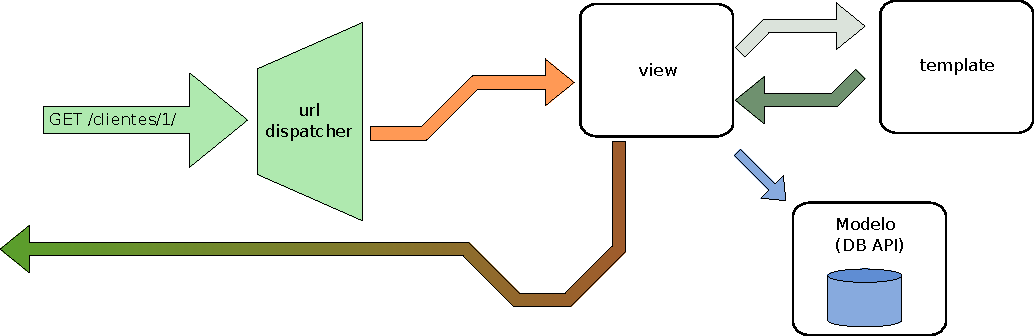
\includegraphics[scale=0.60]{img/django_simple_mtv.pdf}
\caption{Estruccura báisca de Django}\label{fig:erptsqfit}
\end{figure}
  

Django como framework de desarrollo consiste en un  conjunto de utilidades 
de consola que permiten crear y manipular proyectos y aplicaciones.

\subsection*{Estructura de un proyecto}
%%Django implementa una estructura \emph{modelo}, \emph{vista}, \emph{plantilla}.
%% o MTV por sus siglas en inglés (model, view, template).
Un proyecto funciona como un contenedor de aplicaciones que ser rigen bajo
la misma base de datos, los mismos templates y las mismas clases de middleware.

Una aplicación es un paquete que contiene al menos los módulos \textbf{models.py} y \textbf{views.py}, 
y generalmente suele agregarse un módulo \textbf{urls.py}.




%  Dentro de estas utilidades encontramos 
% un servidor standalone de desarrollo para probar los proyectos, creación de 
% tablas a partir de los modelos del mapeador objeto-relacional, realizar 
% volcado y carga de datos (\emph{fixtures}), ejecución de pruebas basadas 
% en test de unidad, entre otras.

Un \label{django:proyecto}{proyecto} Django consite en 3 módulos\footnote{Un módulo en Python, es un
archivo con extensión .py} básicos:
\subsubsection*{Módulo manage.py}
  Esta es la interfase con el framework. Este módulo permite crear aplicaciones,
testear que los modelos de una aplicación estén bien definidos (validación),
iniciar el servidor de desarrollo, crar volcados de la base de datos y restaurarlos
restaurarlos (\emph{fixtures}, utilizados en casos de pruebas y para precarga
de datos conocidos).

\subsubsection*{Módulo settings.py}
  El módulo \emph{settings} define la configuración transversal
a las aplicaciones de usuario. En este módulo no se suelen definir más que constantes.
Dentro de estas constantes encontramos la base de datos sobre la cual trabaja el ORM, 
el(los) directorio(s) de las plantillas, las clases middleware,
ubicación de los medios estáticos\footnote{
Un medio estático es todo contenido que no se genera dinámicamente, como imágenes, 
liberías de javascript, contenido para embeber como archivos multimedia u elementos}.
En este módulo se defnien la lista de aplicaciones instaladas.

\subsubsection*{Módulo urls.py}
  Este módulo define las asociacines entre las URL y las funciones (vistas) que las
atienden. Para generar código más modular, django permite delegar urls que cumplan
con cierto patrón a un otro módulo. Típicamente este módulo se llama también urls y 
es parte de una aplicación (Ej: tratar todo lo lo que comience con \textbf{/clientes/} con el módulo
\textbf{mi\_proyecto.mi\_aplicacion.urls}).

Una \emph{expresión regular} es una forma de definir un patrón en una cadena. Mediante
ésta técnica se realizan validaciones y búsquedas de elementos en cadenas. En python
se define además una forma de otorgarle un alias a los elementos buscaods (en contraposición
a la forma tradicional que utiliza un índice numérico).
Esta particularidad de las expresiones regulares ha sido explotada para la asociación
de las URLs a las funciones que las atienden.
Cuando el cliente realiza accede a una URL dentro de un proyecto django, esta es checkeada
contra cada patrón definido como url, en caso de éxito, se ejecuta la función asociada o vista.
Si la expresión regualar tiene definido gurpos nombrados, cada subcadena pasa a ser argumento

pasan a ser argumentos de la vista, es decir, cada grupo nombrado, pasa a ser argumento
de la función asociada.

\subsection*{Elementos de una aplicación Django}

Una aplicación consiste en 2 módulos fundamentales.
\subsubsection*{Módulo models.py}
En este módulo se definien los modelos.

\subsubsection*{Módulo views.py}
En este módulo se definen las viastas. Una vista es una función que recibe como primer
argumento un objeto HttpRequest\footnote{
\href{http://docs.djangoproject.com/en/dev/ref/request-response/\#httprequest-objects}
{Documentación oficial sobre HttpRequest en djangoproject.com}}, el cual encapsula la información preveniente del request, 
como el método (GET, POST), los elementos de la query http.
\begin{figure}[htp]
\centering
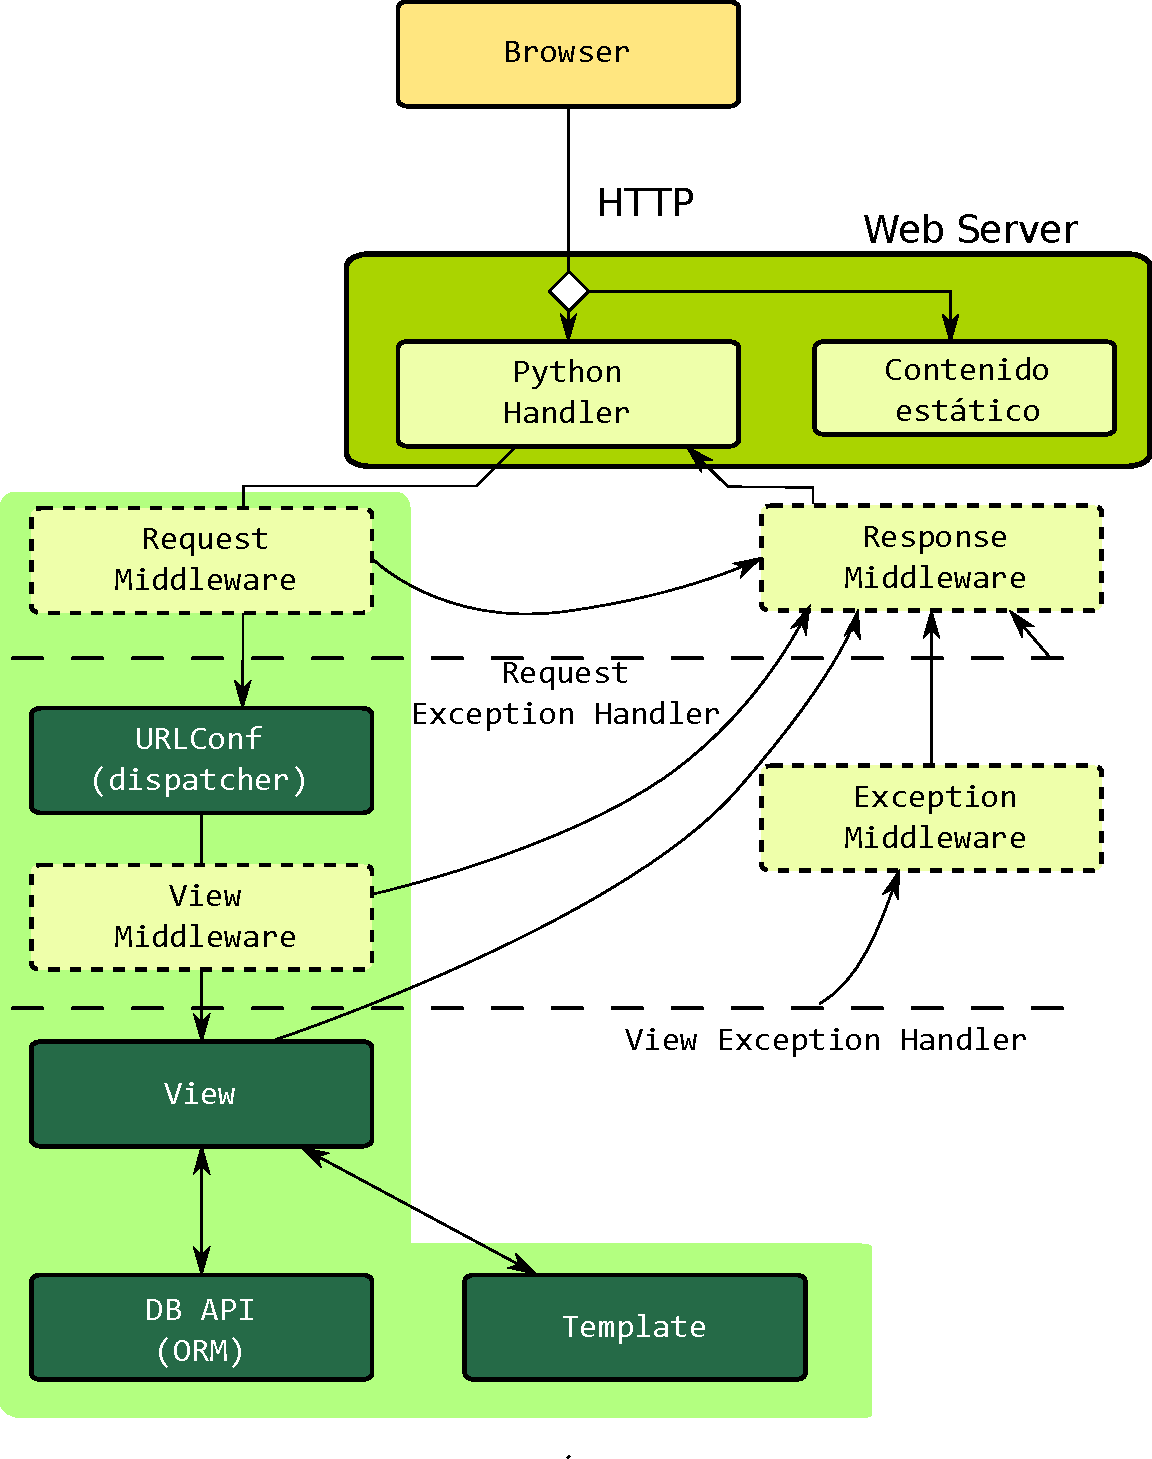
\includegraphics[scale=0.40]{img/django_strucure.pdf}
\caption{Esquema de flujo de una aplicación Django}\label{fig:erptsqfit}
\end{figure}


\chapter{El cliente Web}

\section{Google Gears}
Google Gears es un plug-in para los navegadores: Mozilla Firefox, Internet
Explorer y IE Mobile, Opera y Opera Mobile, Safari y Google Chrome. Gears es
un proyecto de código abierto y añade 3 componentes básicos al navegador.
\begin{itemize}
  \item {\textbf{Local Server:} Permite almacenar en caché y proporcionar
  recursos de aplicaciones (HTML, JavaScript, imágenes, etc.) de forma local. }
  \item {\textbf{Database:} Permite almacenar datos localmente en una base
  de datos relacional en la que se pueden realizar búsquedas. }
  \item { \textbf{Worker Pool:} Permite realizar tareas que utilizan
  intensamente el CPU de forma similar a ``procesos'' en un sistema operativo, de manera de que el 
  las aplicaciones tengan mejor respuesta.}
\end{itemize}
Estos componentes estan enfocados en permitir al programador de aplicaciones web
ejecutar sus aplicaciones cuando el navegador no está conectado al servidor.

Vale aclarar que la aplicación debe ser transferida de manera previa al cliente.

\subsection{Componentes adicionales de Google Gears}
A partir de la versión 0.4 del Gears
\begin{itemize}
  \item{API para GIS, que permite acceder a la posición geográfica del usuario.}
  \item {El API Blob, que permite gestionar bloques de datos binarios.}
  \item {Accede a archivos en el equipo cliente a través del API de Google
  Desktop.}
  \item {Permite enviar y recibir Blobs con el API HttpRequest.}
  \item {Localización de los cuadros de diálogo de Gears en varios idiomas.}  
\end{itemize}



\section{Estructura de un navegador}

\section{Evolución del lenguaje en el cliente}
\subsection{JavaScript}

\section{Propuesta de extensión de Google Gears}
\section{Propuesta de extensión y aprovechamiento de los avances en cliente}
% Acá ponemos por que geraquía de clases

El desarrollo de un framework en javascript que funcione del lado del cliente presupone gran cantidad de codigo
viajando de un lado al otro de la conexion. Previendo basicamente este postulado desarrollamos una libreria
que brinde el soporte a los requerimentos mas basicos.
Esta librería contituye la base para posteriores contrucciones mas complejas en el ciente y auna herramientas
que simplifican el desarrollo client-side.

\section{Modulos}
Undo de los principales inconvenientes a los que protopy da solucion es a la inclucion dinamica de funcionalidad bajo demanda,
esto es logrado mediante los modulos.
Basicamente un modulo en un archivo con codigo javascript que recide en el servidor y es obtenido y ejecutado en el cliente.

\begin{lstlisting}[style=javascript,label=estructura-modulo,caption=Estructura de un modulo]
//Archivo: tests/module.js
require('event');

var h1 = $('titulo');

function set_texto(txt) {
    h1.update(txt);
}

function get_texto() {
    return h1.innerHTML;
}

event.connect($('titulo'), 'click', function(event) {
    alert('El texto es: ' + event.target.innerHTML);
});

publish({
    set_texto: set_texto,
    get_texto: get_texto
});
\end{lstlisting}

\begin{lstlisting}[style=consola,label=estructura-modulo-test,caption=Test]
>>> require('tests.module')
GET http://localhost:8080/tests/protopy/module.js
Object __file__=/tests/protopy/module.js
>>> module.get_texto()
"Test de modulo"
>>> module.set_texto('Un titulo')
>>> require('tests.module', 'get_texto')
get_texto()
>>> get_texto()
"Un titulo"
>>> require('tests.module', '*')
>>> set_texto('Hola luuu!!!')
>>> get_texto()
"Hola luuu!!!"
\end{lstlisting}

\subsection{builtin}
\subsection{sys}
\subsection{exception}
\subsection{event}
\subsection{timer}
\subsection{ajax}
\subsection{dom}

\section{sys}
\subsection*{version}
version: 0.8,
\subsection*{browser}
	browser: {
	    IE:     !!(window.attachEvent && navigator.userAgent.indexOf('Opera') === -1),
	    Opera:  navigator.userAgent.indexOf('Opera') > -1,
	    WebKit: navigator.userAgent.indexOf('AppleWebKit/') > -1,
	    Gecko:  navigator.userAgent.indexOf('Gecko') > -1 && navigator.userAgent.indexOf('KHTML') === -1,
	    MobileSafari: !!navigator.userAgent.match(/Apple.*Mobile.*Safari/),
	    features: {
		XPath: !!document.evaluate,
		SelectorsAPI: !!document.querySelector,
		ElementExtensions: !!window.HTMLElement,
		SpecificElementExtensions: document.createElement('div')['__proto__'] &&
						document.createElement('div')['__proto__'] !==
						document.createElement('form')['__proto__']
	      Gears = !!get_gears() || false;

	    }
	},
\subsection*{get\_gears}
get\_gears: get_gears,
\subsection*{register\_path}
register\_path: function(module, path)
\subsection*{module\_url}
module\_url: function(name, postfix) {
\subsection*{modules}
modules: ModuleManager.modules,
\subsection*{paths}
paths: ModuleManager.paths

\section{exception}
var exception = ModuleManager.create('exceptions', 'built-in', {
        Exception: Exception,
        AssertionError: type('AssertionError', Exception),
        AttributeError: type('AttributeError', Exception),
        LoadError: type('LoadError', Exception),
        KeyError: type('KeyError', Exception),
        NotImplementedError: type('NotImplementedError', Exception),
        TypeError: type('TypeError', Exception),
        ValueError: type('ValueError', Exception),
    });

\section{event}
\subsection*{connect}
connect(object, event, context, method) {
\subsection*{disconnect}
disconnect(handle) {
\subsection*{subscribe}
subscribe(topic, context, method) {
\subsection*{unsubscribe}
unsubscribe(handle) {
\subsection*{publish}
publish(topic, args) {
\subsection*{connectpublisher}
connectpublisher(topic, obj, event) {
\subsection*{fixevent}
fixevent: function(){},
\subsection*{stopevent}
stopevent: function(){},
\subsection*{keys}
keys: { BACKSPACE: 8, TAB: 9, CLEAR: 12, ENTER: 13, SHIFT: 16, CTRL: 17, ALT: 18, PAUSE: 19, CAPS_LOCK: 20, 
		    ESCAPE: 27, SPACE: 32, PAGE_UP: 33, PAGE_DOWN: 34, END: 35, HOME: 36, LEFT_ARROW: 37, UP_ARROW: 38,
		    RIGHT_ARROW: 39, DOWN_ARROW: 40, INSERT: 45, DELETE: 46, HELP: 47, LEFT_WINDOW: 91, RIGHT_WINDOW: 92,
		    SELECT: 93, NUMPAD_0: 96, NUMPAD_1: 97, NUMPAD_2: 98, NUMPAD_3: 99, NUMPAD_4: 100, NUMPAD_5: 101,
		    NUMPAD_6: 102, NUMPAD_7: 103, NUMPAD_8: 104, NUMPAD_9: 105, NUMPAD_MULTIPLY: 106, NUMPAD_PLUS: 107,
		    NUMPAD_ENTER: 108, NUMPAD_MINUS: 109, NUMPAD_PERIOD: 110, NUMPAD_DIVIDE: 111, F1: 112, F2: 113, F3: 114,
		    F4: 115, F5: 116, F6: 117, F7: 118, F8: 119, F9: 120, F10: 121, F11: 122, F12: 123, F13: 124, 
		    F14: 125, F15: 126, NUM_LOCK: 144, SCROLL_LOCK: 145 }
    });

\section{timer}
\subsection*{setTimeout}
setTimeout: window.setTimeout,
\subsection*{setInterval}
setInterval: window.setInterval,
\subsection*{clearTimeout}
clearTimeout: window.clearTimeout,
\subsection*{delay}
delay: function(f) {
\subsection*{defer}
defer: function(f) {

\section{ajax}
\subsection*{Request}
new Request: Request,
\subsection*{Response}
new Response: Response,
\subsection*{toQueryParams}
toQueryParams(string, separator) \rightarrow object
\subsection*{toQueryString}
toQueryString(params) -> string

\section{dom}
\subsection*{query}
query: query,

\section{builtin}
\subsection*{publish}
publish(object)
\subsection*{require}
require(module[, object...]) -> module | object
\subsection*{\$}
\$(id) -> HTMLElement
\$(id ...) -> [HTMLElement...]
\subsection*{\$\$}
\$\$(cssRule) -> [HTMLElement...]
\subsection*{type, El constructor de tipos}
type(name, [base...] [, forType ], forPrototype) -> newType

Como ya se menciono anteriormente javascript es un lenguaje orientado a prototipos, para acercarnos un poco a la programacion
de objetos, utilizamos una funcion constructora de tipos o clases a la que denominamos “type”.
\begin{lstlisting}[style=javascript,label=definicion-de-tipos,caption=Definicion de tipos]
var Animal = type('Animal', object, {
    contador: 0,
}, {
    __init__: function(especie) {
	this.especie = especie;
	this.orden = Animal.contador++;
    }
});

var Terrestre = type('Terrestre', Animal, {
    caminar: function() {
	console.log(this.especie + ' caminando');
    }
});

var Acuatico = type('Acuatico', Animal, {
    nadar: function() {
	console.log(this.especie + ' nadando');
    }
});

var Anfibio = type('Anfibio', [Terrestre, Acuatico]);

var Piton = type('Piton', Terrestre, {
    __init__: function(nombre) {
	super(Terrestre, this).__init__(this.__name__);
	this.nombre = nombre;
    },
    caminar: function() {
	throw new Exception(this.especie + ' no camina');
    },
    reptar: function() {
	console.log(this.nombre + ' la ' + this.especie.toLowerCase() + ' esta reptando');
    }
});

var doris = new Piton('Doris');
var ballena = new Acuatico('Ballena');
var rana = new Anfibio('Rana');
\end{lstlisting}

\begin{lstlisting}[style=consola,label=definicion-de-tipos-test,caption=Test]
>>> doris
window.Piton especie=Piton orden=0 nombre=Doris __name__=Piton
>>> rana
window.Anfibio especie=Rana orden=2 __name__=Anfibio
>>> isinstance(rana, Terrestre)
true
>>> isinstance(doris, Animal)
true
>>> issubclass(Anfibio, Acuatico)
true
>>> issubclass(Piton, Animal)
true
>>> doris.caminar()
Exception: Piton no camina args=[1] message=Piton no camina
>>> doris.reptar()
Doris la piton esta reptando
\end{lstlisting}

\subsection*{extend}
extend(destiny, source) -> alteredDestiny
\subsection*{super}
super(destiny, source) -> alteredDestiny
\subsection*{isundefined}
isundefined(destiny, source) -> alteredDestiny
\subsection*{isinstance}
isundefined(destiny, source) -> alteredDestiny
\subsection*{issubclass}
issubclass(destiny, source) -> alteredDestiny
\subsection*{Arguments}
new Arguments(destiny, source) -> alteredDestiny
\subsection*{Template}
new Template(destiny, source) -> alteredDestiny
\subsection*{Dict}
new Dict(destiny, source) -> alteredDestiny
\subsection*{Set}
new Set(destiny, source) -> alteredDestiny
\subsection*{hash}
hash(destiny, source) -> alteredDestiny
\subsection*{id}
id(destiny, source) -> alteredDestiny
\subsection*{getattr}
getattr(destiny, source) -> alteredDestiny
\subsection*{setattr}
setattr(destiny, source) -> alteredDestiny
\subsection*{hasattr}
hasattr(destiny, source) -> alteredDestiny
\subsection*{assert}
assert(destiny, source) -> alteredDestiny
\subsection*{bool}
bool(destiny, source) -> alteredDestiny
\subsection*{callable}
callable(destiny, source) -> alteredDestiny
\subsection*{chr}
chr(destiny, source) -> alteredDestiny
\subsection*{ord}
ord(destiny, source) -> alteredDestiny
\subsection*{bisect}
bisect(destiny, source) -> alteredDestiny
\subsection*{equal}
equal(destiny, source) -> alteredDestiny
\subsection*{nequal}
nequal(destiny, source) -> alteredDestiny
\subsection*{number}
number(destiny, source) -> alteredDestiny
\subsection*{flatten}
flatten(destiny, source) -> alteredDestiny
\subsection*{include}
include(destiny, source) -> alteredDestiny
\subsection*{len}
len(destiny, source) -> alteredDestiny
\subsection*{array}
array(iterable) -> [element...]
\subsection*{print}
print(destiny, source) -> alteredDestiny
\subsection*{range}
range(destiny, source) -> alteredDestiny
\subsection*{string}
string(destiny, source) -> alteredDestiny
\subsection*{values}
values(object) -> [value...]
\subsection*{keys}
keys(object) -> [key...]
\subsection*{items}
items(destiny, source) -> alteredDestiny
\subsection*{inspect}
inspect(destiny, source) -> alteredDestiny
\subsection*{unique}
unique(destiny, source) -> alteredDestiny
\subsection*{xrange}
xrange(destiny, source) -> alteredDestiny
\subsection*{zip}
zip(destiny, source) -> alteredDestiny

santiago del estero norte 727, tiene un pino grande

\section{Extendiendo Javascript}
\subsection{String}
\subsubsection*{gsub}
gsub(pattern, replacement) -> string
\subsubsection*{sub}
sub(pattern, replacement[, count = 1]) -> string
\subsubsection*{subs}
subs(pattern, replacement) -> string
\subsubsection*{format}
format(pattern, replacement) -> string
\subsubsection*{inspect} 
inspect(use_double_quotes) -> string
\subsubsection*{truncate}
truncate(length, truncation) -> string
\subsubsection*{strip}
strip() -> string
\subsubsection*{striptags}
striptags() -> string
\subsubsection*{stripscripts}
stripscripts() -> string
\subsubsection*{extractscripts}
extractscripts() -> string
\subsubsection*{evalscripts}
evalscripts() -> string
\subsubsection*{escapeHTML}
escapeHTML() -> string
\subsubsection*{unescapeHTML}
unescapeHTML() -> string
\subsubsection*{succ}
succ() -> string
\subsubsection*{times}
times(count[, separator = '']) -> string
\subsubsection*{camelize}
camelize() -> string
\subsubsection*{capitalize}
capitalize() -> string
\subsubsection*{underscore}
underscore() -> string
\subsubsection*{dasherize}
dasherize() -> string
\subsubsection*{startswith}
startswith(pattern) -> string
\subsubsection*{endswith}
endswith(pattern) -> string
\subsubsection*{blank}
blank() -> string

\subsection{Number}
\subsubsection*{format}
format(f, radix) -> string

\subsection{Date}
\subsubsection*{toISO8601}
toISO8601() -> string

\subsection{Element}
\subsubsection*{visible}
visible() {
\subsubsection*{toggle}
toggle() {
\subsubsection*{hide}
hide() {
\subsubsection*{show}
show() {
\subsubsection*{remove}
remove() {
\subsubsection*{update}
update(content) {
\subsubsection*{insert}
insert(insertions) {
\subsubsection*{select}
select(selector) {

\subsection{Forms}
\subsubsection*{disable}
disable() {
\subsubsection*{enable}
enable() {
\subsubsection*{serialize}
serialize() {

\subsection{Forms.Element}
\subsubsection*{serialize}
serialize() {
\subsubsection*{get\_value}
get\_value() {
\subsubsection*{set\_value}
set\_value(value) {
\subsubsection*{clear}
clear() {
\subsubsection*{present}
present() {
\subsubsection*{activate}
activate() {
\subsubsection*{disable}
disable() {
\subsubsection*{enable}
enable() {
\chapter{Propuesta de framework MTV en el cliente}

\section{que}
El desarrollo de un framework en JavaScript funcionando dentro del navegador
Firefox, deja entrever una gran cantidad de detalles que no resultan triviales
al momento de desarrollar.
\begin{itemize}
 \item Se requieren varias lineas de codigo para implementar un framework.
 \item Como llega el codigo al navegador y se inicia su ejecucion.
 \item La cara visible o vista debe ser fasilmente manipulable por la aplicacion
de usuario.
 \item Como los datos generados en el cliente son informados al servidor.
 \item El framework debe brindar soporte a la aplicacion de usuario de una forma
natural y transparente.
 \item Se debe promover al reuso y la extension de funcionalidad del framework.
 \item Como se ponen en marcha los mecanimos o acciones que la aplicacion de
usuario define.
 \item ...
\end{itemize} 
Si bien el desarrollo de Protopy se mantuvo en paralelo a la del
framework, existen aspectos basicos a los que esta brinda soporte y permiten
presentarla en un apartado separado como una ''Libreria JavaScript''.

\textit{proto}type + \textit{py}thon = \textit{protopy}

``La creación nace del caos'', Protopy no escapa a esta afirmacion y nace de la
integracion de la libreria Prototype con las primeras funciones para lograr
la modularizacion; con el correr de las lineas de codigo\footnote{Forma en que
los informaticos miden el paso del tiempo} el desarrollo del framework convierte
el enfoque inicial en poco sustentable, requiriendo este de funciones mas
Python-compatibles se desecha buena parte de la libreria base y se continua con
un enfoque mas ``pythonico''.

En este capitulo se explicara como Protopy da solucion a los items expuestos y
terminando una definicion.

\textit{Protopy es una libreria JavaScript para el desarrollo de aplicaciones
web dinamicas. Aporta un enfoque modular para la inclusión de código,
orientación a objetos, manejo de AJAX, DOM y eventos.}

% llamaron para papa, llamar a este numero 0800-666-1153 rio 
\section{como}

El desarrollo de un framework en javascript que funcione del lado del cliente
presupone gran cantidad de codigo
viajando de un lado al otro de la conexion. Previendo basicamente este postulado
desarrollamos una libreria
que brinde el soporte a los requerimentos mas basicos.
Esta librería contituye la base para posteriores contrucciones mas complejas en
el ciente y auna herramientas
que simplifican el desarrollo client-side.


\section{Modulos}
Undo de los principales inconvenientes a los que protopy da solucion es a la
inclucion dinamica de funcionalidad bajo demanda,
esto es logrado mediante los modulos.
Basicamente un modulo en un archivo con codigo javascript que recide en el
servidor y es obtenido y ejecutado en el cliente.


%----------------------------------------------------------------------------
% Capitulo 
%----------------------------------------------------------------------------
\chapter{Integración y metodología de desarrollo con framework web}
\section{Mecanismos de extension de Django}

\subsection{Comandos Personalizados}


% La interacción con Django se realiza mediante comandos CLI\footnote{
% \emph{Command Line Interfece}, interfase de linea de comandos, tamién
% conocidos como comandos de consola o  terminal}. Django posee un set
% de comandos que permiten crear proyectos, crear aplicaciones, sincronizar
% la definición del modelo con la base de datos, volcado y recuperación de datos,
% ejecución del servidor de desarrollo entre otras funcionalidades.

Para poder realizar extensiones sobre la funcionalidad de Django sus
desarrolladores han añadido la posibilidad de crear comandos
personalizados. Un comando personalizado se define en un módulo, dentro
de una aplicación y es ejecutado de manrera similar a cualquer 
otro comando provisto por el framework(como 
\emph{syncdb}, \emph{runserver}, \emph{dumpdata}).

De igual manera que los comandos provistos por el framework, los comandos
personalizados son ejecutados mediante el script de administración
de proyecto \emph{manage.py} o \emph{django-admin.py}.

Un comando se define dentro de una aplicación. No existen comandos a nivel
proyecto. Para que estos comandos sean detectados por el módulo de
administración de poryectos deben  respetar la siguiente estructura dentro del
directorio de la aplicación 
\begin{verbatim}
management/
    __init__.py
    commands/
        __init__.py
        mi_comando.py
\end{verbatim}

Además la aplicación debe estar incluida en \textbf{INSTALLED\_APPS}
dentro de el módulo de configuración de proyecto \textbf{settings.py}.

\begin{lstlisting}[style=python,
		   label=basic-django-command,
		   caption=Comando personalizado básico en Django]

from django.core.management.base import NoArgsCommand

class Command(NoArgsCommand):
  help = '''Descripción del comando '''
  def handle_noargs(self, **options):
    print "Soy un comando personalizado"

\end{lstlisting}

Desde el punto de vista del lenguaje, la creación de un comando es la creación
de un módulo management.commands.nombre\_comando, en el cual se extiende 
a alguna clase base Command (que se encuentran en django.core.management.base).

Las clases base diponible son NoArgsCommand, para la imeplentación de comandos
que no reciben argumentos; AppLabelCommand para la implementación de comandos
que reciben como argumento el nombre de una aplicación instalada y 

\section{Integración}
Se decide utilizar un ManagedStore para almacenar la aplicación y los médios
estáticos y uno para almacenar el Framework.

 
\section{Convivencia}

\subsection{Modos de trabajo}
Los distinotos modos de trabajo de la aplicacion son:
\subsubsection{Estado online sin soporte offline}
En este modo la aplicacion trabaja directamente sobre el servidor de aplicacion y depende completamente de una conexion.
Al activar e implementar el soporte offline para nuestra aplicacion, en el servidor; el cliente debe ser conciente de este cambio y pasar a soportar los modos.
\subsubsection{Estado online con soporte offline}
\subsubsection{Estado offline con soporte offline}

\chapter{Lineas futuras}
\section{Sitio de administración}
Django se caracteriza por brindar una aplicación (\textit{django.contrib.admin})
de admnistración que permite realizar CRUD (\textit{Create}, \textit{Retrieve}
\textit{Update}, \textit{Delete}) sobre los modelos de las aplicaciones de
usuario, interactuando con la aplicación \textit{django.contrib.auth} que provee
usuarios, grupos y permisos.
 
\section{Historial de navegación}

\section{Workers con soporte para Javascript 1.7}
Google Gears provee un mecanismo de ejecución de código en el cliente de manera
concurrente llamado Worker Pool. De esta manera tareas que demandan tiempo de
CPU pueden ser envaidas a segundo plano, de manera de no entorpecer el refresco 
de la GUI.
Una caractersística de los worker pools, es que se ejecutan en un ámbito de 
nombres diferente al del ``hilo principal''. Es decir, existe encapsulamiento
de su estado.
 
\appendix
El desarrollo de un framework en javascript que funcione del lado del cliente presupone gran cantidad de codigo
viajando de un lado al otro de la conexion. Previendo basicamente este postulado desarrollamos una libreria
que brinde el soporte a los requerimentos mas basicos.
Esta librería contituye la base para posteriores contrucciones mas complejas en el ciente y auna herramientas
que simplifican el desarrollo client-side.

\section{Modulos}
Undo de los principales inconvenientes a los que protopy da solucion es a la inclucion dinamica de funcionalidad bajo demanda,
esto es logrado mediante los modulos.
Basicamente un modulo en un archivo con codigo javascript que recide en el servidor y es obtenido y ejecutado en el cliente.

\begin{lstlisting}[style=javascript,label=estructura-modulo,caption=Estructura de un modulo]
//Archivo: tests/module.js
require('event');

var h1 = $('titulo');

function set_texto(txt) {
    h1.update(txt);
}

function get_texto() {
    return h1.innerHTML;
}

event.connect($('titulo'), 'click', function(event) {
    alert('El texto es: ' + event.target.innerHTML);
});

publish({
    set_texto: set_texto,
    get_texto: get_texto
});
\end{lstlisting}

\begin{lstlisting}[style=consola,label=estructura-modulo-test,caption=Test]
>>> require('tests.module')
GET http://localhost:8080/tests/protopy/module.js
Object __file__=/tests/protopy/module.js
>>> module.get_texto()
"Test de modulo"
>>> module.set_texto('Un titulo')
>>> require('tests.module', 'get_texto')
get_texto()
>>> get_texto()
"Un titulo"
>>> require('tests.module', '*')
>>> set_texto('Hola luuu!!!')
>>> get_texto()
"Hola luuu!!!"
\end{lstlisting}

\subsection{builtin}
\subsection{sys}
\subsection{exception}
\subsection{event}
\subsection{timer}
\subsection{ajax}
\subsection{dom}

\section{sys}
\subsection*{version}
version: 0.8,
\subsection*{browser}
	browser: {
	    IE:     !!(window.attachEvent && navigator.userAgent.indexOf('Opera') === -1),
	    Opera:  navigator.userAgent.indexOf('Opera') > -1,
	    WebKit: navigator.userAgent.indexOf('AppleWebKit/') > -1,
	    Gecko:  navigator.userAgent.indexOf('Gecko') > -1 && navigator.userAgent.indexOf('KHTML') === -1,
	    MobileSafari: !!navigator.userAgent.match(/Apple.*Mobile.*Safari/),
	    features: {
		XPath: !!document.evaluate,
		SelectorsAPI: !!document.querySelector,
		ElementExtensions: !!window.HTMLElement,
		SpecificElementExtensions: document.createElement('div')['__proto__'] &&
						document.createElement('div')['__proto__'] !==
						document.createElement('form')['__proto__']
	      Gears = !!get_gears() || false;

	    }
	},
\subsection*{get\_gears}
get\_gears: get_gears,
\subsection*{register\_path}
register\_path: function(module, path)
\subsection*{module\_url}
module\_url: function(name, postfix) {
\subsection*{modules}
modules: ModuleManager.modules,
\subsection*{paths}
paths: ModuleManager.paths

\section{exception}
var exception = ModuleManager.create('exceptions', 'built-in', {
        Exception: Exception,
        AssertionError: type('AssertionError', Exception),
        AttributeError: type('AttributeError', Exception),
        LoadError: type('LoadError', Exception),
        KeyError: type('KeyError', Exception),
        NotImplementedError: type('NotImplementedError', Exception),
        TypeError: type('TypeError', Exception),
        ValueError: type('ValueError', Exception),
    });

\section{event}
\subsection*{connect}
connect(object, event, context, method) {
\subsection*{disconnect}
disconnect(handle) {
\subsection*{subscribe}
subscribe(topic, context, method) {
\subsection*{unsubscribe}
unsubscribe(handle) {
\subsection*{publish}
publish(topic, args) {
\subsection*{connectpublisher}
connectpublisher(topic, obj, event) {
\subsection*{fixevent}
fixevent: function(){},
\subsection*{stopevent}
stopevent: function(){},
\subsection*{keys}
keys: { BACKSPACE: 8, TAB: 9, CLEAR: 12, ENTER: 13, SHIFT: 16, CTRL: 17, ALT: 18, PAUSE: 19, CAPS_LOCK: 20, 
		    ESCAPE: 27, SPACE: 32, PAGE_UP: 33, PAGE_DOWN: 34, END: 35, HOME: 36, LEFT_ARROW: 37, UP_ARROW: 38,
		    RIGHT_ARROW: 39, DOWN_ARROW: 40, INSERT: 45, DELETE: 46, HELP: 47, LEFT_WINDOW: 91, RIGHT_WINDOW: 92,
		    SELECT: 93, NUMPAD_0: 96, NUMPAD_1: 97, NUMPAD_2: 98, NUMPAD_3: 99, NUMPAD_4: 100, NUMPAD_5: 101,
		    NUMPAD_6: 102, NUMPAD_7: 103, NUMPAD_8: 104, NUMPAD_9: 105, NUMPAD_MULTIPLY: 106, NUMPAD_PLUS: 107,
		    NUMPAD_ENTER: 108, NUMPAD_MINUS: 109, NUMPAD_PERIOD: 110, NUMPAD_DIVIDE: 111, F1: 112, F2: 113, F3: 114,
		    F4: 115, F5: 116, F6: 117, F7: 118, F8: 119, F9: 120, F10: 121, F11: 122, F12: 123, F13: 124, 
		    F14: 125, F15: 126, NUM_LOCK: 144, SCROLL_LOCK: 145 }
    });

\section{timer}
\subsection*{setTimeout}
setTimeout: window.setTimeout,
\subsection*{setInterval}
setInterval: window.setInterval,
\subsection*{clearTimeout}
clearTimeout: window.clearTimeout,
\subsection*{delay}
delay: function(f) {
\subsection*{defer}
defer: function(f) {

\section{ajax}
\subsection*{Request}
new Request: Request,
\subsection*{Response}
new Response: Response,
\subsection*{toQueryParams}
toQueryParams(string, separator) \rightarrow object
\subsection*{toQueryString}
toQueryString(params) -> string

\section{dom}
\subsection*{query}
query: query,

\section{builtin}
\subsection*{publish}
publish(object)
\subsection*{require}
require(module[, object...]) -> module | object
\subsection*{\$}
\$(id) -> HTMLElement
\$(id ...) -> [HTMLElement...]
\subsection*{\$\$}
\$\$(cssRule) -> [HTMLElement...]
\subsection*{type, El constructor de tipos}
type(name, [base...] [, forType ], forPrototype) -> newType

Como ya se menciono anteriormente javascript es un lenguaje orientado a prototipos, para acercarnos un poco a la programacion
de objetos, utilizamos una funcion constructora de tipos o clases a la que denominamos “type”.
\begin{lstlisting}[style=javascript,label=definicion-de-tipos,caption=Definicion de tipos]
var Animal = type('Animal', object, {
    contador: 0,
}, {
    __init__: function(especie) {
	this.especie = especie;
	this.orden = Animal.contador++;
    }
});

var Terrestre = type('Terrestre', Animal, {
    caminar: function() {
	console.log(this.especie + ' caminando');
    }
});

var Acuatico = type('Acuatico', Animal, {
    nadar: function() {
	console.log(this.especie + ' nadando');
    }
});

var Anfibio = type('Anfibio', [Terrestre, Acuatico]);

var Piton = type('Piton', Terrestre, {
    __init__: function(nombre) {
	super(Terrestre, this).__init__(this.__name__);
	this.nombre = nombre;
    },
    caminar: function() {
	throw new Exception(this.especie + ' no camina');
    },
    reptar: function() {
	console.log(this.nombre + ' la ' + this.especie.toLowerCase() + ' esta reptando');
    }
});

var doris = new Piton('Doris');
var ballena = new Acuatico('Ballena');
var rana = new Anfibio('Rana');
\end{lstlisting}

\begin{lstlisting}[style=consola,label=definicion-de-tipos-test,caption=Test]
>>> doris
window.Piton especie=Piton orden=0 nombre=Doris __name__=Piton
>>> rana
window.Anfibio especie=Rana orden=2 __name__=Anfibio
>>> isinstance(rana, Terrestre)
true
>>> isinstance(doris, Animal)
true
>>> issubclass(Anfibio, Acuatico)
true
>>> issubclass(Piton, Animal)
true
>>> doris.caminar()
Exception: Piton no camina args=[1] message=Piton no camina
>>> doris.reptar()
Doris la piton esta reptando
\end{lstlisting}

\subsection*{extend}
extend(destiny, source) -> alteredDestiny
\subsection*{super}
super(destiny, source) -> alteredDestiny
\subsection*{isundefined}
isundefined(destiny, source) -> alteredDestiny
\subsection*{isinstance}
isundefined(destiny, source) -> alteredDestiny
\subsection*{issubclass}
issubclass(destiny, source) -> alteredDestiny
\subsection*{Arguments}
new Arguments(destiny, source) -> alteredDestiny
\subsection*{Template}
new Template(destiny, source) -> alteredDestiny
\subsection*{Dict}
new Dict(destiny, source) -> alteredDestiny
\subsection*{Set}
new Set(destiny, source) -> alteredDestiny
\subsection*{hash}
hash(destiny, source) -> alteredDestiny
\subsection*{id}
id(destiny, source) -> alteredDestiny
\subsection*{getattr}
getattr(destiny, source) -> alteredDestiny
\subsection*{setattr}
setattr(destiny, source) -> alteredDestiny
\subsection*{hasattr}
hasattr(destiny, source) -> alteredDestiny
\subsection*{assert}
assert(destiny, source) -> alteredDestiny
\subsection*{bool}
bool(destiny, source) -> alteredDestiny
\subsection*{callable}
callable(destiny, source) -> alteredDestiny
\subsection*{chr}
chr(destiny, source) -> alteredDestiny
\subsection*{ord}
ord(destiny, source) -> alteredDestiny
\subsection*{bisect}
bisect(destiny, source) -> alteredDestiny
\subsection*{equal}
equal(destiny, source) -> alteredDestiny
\subsection*{nequal}
nequal(destiny, source) -> alteredDestiny
\subsection*{number}
number(destiny, source) -> alteredDestiny
\subsection*{flatten}
flatten(destiny, source) -> alteredDestiny
\subsection*{include}
include(destiny, source) -> alteredDestiny
\subsection*{len}
len(destiny, source) -> alteredDestiny
\subsection*{array}
array(iterable) -> [element...]
\subsection*{print}
print(destiny, source) -> alteredDestiny
\subsection*{range}
range(destiny, source) -> alteredDestiny
\subsection*{string}
string(destiny, source) -> alteredDestiny
\subsection*{values}
values(object) -> [value...]
\subsection*{keys}
keys(object) -> [key...]
\subsection*{items}
items(destiny, source) -> alteredDestiny
\subsection*{inspect}
inspect(destiny, source) -> alteredDestiny
\subsection*{unique}
unique(destiny, source) -> alteredDestiny
\subsection*{xrange}
xrange(destiny, source) -> alteredDestiny
\subsection*{zip}
zip(destiny, source) -> alteredDestiny

santiago del estero norte 727, tiene un pino grande

\section{Extendiendo Javascript}
\subsection{String}
\subsubsection*{gsub}
gsub(pattern, replacement) -> string
\subsubsection*{sub}
sub(pattern, replacement[, count = 1]) -> string
\subsubsection*{subs}
subs(pattern, replacement) -> string
\subsubsection*{format}
format(pattern, replacement) -> string
\subsubsection*{inspect} 
inspect(use_double_quotes) -> string
\subsubsection*{truncate}
truncate(length, truncation) -> string
\subsubsection*{strip}
strip() -> string
\subsubsection*{striptags}
striptags() -> string
\subsubsection*{stripscripts}
stripscripts() -> string
\subsubsection*{extractscripts}
extractscripts() -> string
\subsubsection*{evalscripts}
evalscripts() -> string
\subsubsection*{escapeHTML}
escapeHTML() -> string
\subsubsection*{unescapeHTML}
unescapeHTML() -> string
\subsubsection*{succ}
succ() -> string
\subsubsection*{times}
times(count[, separator = '']) -> string
\subsubsection*{camelize}
camelize() -> string
\subsubsection*{capitalize}
capitalize() -> string
\subsubsection*{underscore}
underscore() -> string
\subsubsection*{dasherize}
dasherize() -> string
\subsubsection*{startswith}
startswith(pattern) -> string
\subsubsection*{endswith}
endswith(pattern) -> string
\subsubsection*{blank}
blank() -> string

\subsection{Number}
\subsubsection*{format}
format(f, radix) -> string

\subsection{Date}
\subsubsection*{toISO8601}
toISO8601() -> string

\subsection{Element}
\subsubsection*{visible}
visible() {
\subsubsection*{toggle}
toggle() {
\subsubsection*{hide}
hide() {
\subsubsection*{show}
show() {
\subsubsection*{remove}
remove() {
\subsubsection*{update}
update(content) {
\subsubsection*{insert}
insert(insertions) {
\subsubsection*{select}
select(selector) {

\subsection{Forms}
\subsubsection*{disable}
disable() {
\subsubsection*{enable}
enable() {
\subsubsection*{serialize}
serialize() {

\subsection{Forms.Element}
\subsubsection*{serialize}
serialize() {
\subsubsection*{get\_value}
get\_value() {
\subsubsection*{set\_value}
set\_value(value) {
\subsubsection*{clear}
clear() {
\subsubsection*{present}
present() {
\subsubsection*{activate}
activate() {
\subsubsection*{disable}
disable() {
\subsubsection*{enable}
enable() {
\chapter{Propuesta de framework MTV en el cliente}

\section{que}
El desarrollo de un framework en JavaScript funcionando dentro del navegador
Firefox, deja entrever una gran cantidad de detalles que no resultan triviales
al momento de desarrollar.
\begin{itemize}
 \item Se requieren varias lineas de codigo para implementar un framework.
 \item Como llega el codigo al navegador y se inicia su ejecucion.
 \item La cara visible o vista debe ser fasilmente manipulable por la aplicacion
de usuario.
 \item Como los datos generados en el cliente son informados al servidor.
 \item El framework debe brindar soporte a la aplicacion de usuario de una forma
natural y transparente.
 \item Se debe promover al reuso y la extension de funcionalidad del framework.
 \item Como se ponen en marcha los mecanimos o acciones que la aplicacion de
usuario define.
 \item ...
\end{itemize} 
Si bien el desarrollo de Protopy se mantuvo en paralelo a la del
framework, existen aspectos basicos a los que esta brinda soporte y permiten
presentarla en un apartado separado como una ''Libreria JavaScript''.

\textit{proto}type + \textit{py}thon = \textit{protopy}

``La creación nace del caos'', Protopy no escapa a esta afirmacion y nace de la
integracion de la libreria Prototype con las primeras funciones para lograr
la modularizacion; con el correr de las lineas de codigo\footnote{Forma en que
los informaticos miden el paso del tiempo} el desarrollo del framework convierte
el enfoque inicial en poco sustentable, requiriendo este de funciones mas
Python-compatibles se desecha buena parte de la libreria base y se continua con
un enfoque mas ``pythonico''.

En este capitulo se explicara como Protopy da solucion a los items expuestos y
terminando una definicion.

\textit{Protopy es una libreria JavaScript para el desarrollo de aplicaciones
web dinamicas. Aporta un enfoque modular para la inclusión de código,
orientación a objetos, manejo de AJAX, DOM y eventos.}

% llamaron para papa, llamar a este numero 0800-666-1153 rio 
\section{como}

El desarrollo de un framework en javascript que funcione del lado del cliente
presupone gran cantidad de codigo
viajando de un lado al otro de la conexion. Previendo basicamente este postulado
desarrollamos una libreria
que brinde el soporte a los requerimentos mas basicos.
Esta librería contituye la base para posteriores contrucciones mas complejas en
el ciente y auna herramientas
que simplifican el desarrollo client-side.


\section{Modulos}
Undo de los principales inconvenientes a los que protopy da solucion es a la
inclucion dinamica de funcionalidad bajo demanda,
esto es logrado mediante los modulos.
Basicamente un modulo en un archivo con codigo javascript que recide en el
servidor y es obtenido y ejecutado en el cliente.
\chapter{MIME}

\textbf{MIME} \label{mime}(\textit{\textbf{M}ultipurpose \textbf{I}nternet \textbf{M}ail \textbf{E}xtensions}), 
(Extensiones de Correo de Internet Multipropósito), son una serie de
convenciones o especificaciones dirigidas a que se puedan intercambiar a través
de Internet todo tipo de archivos (texto, audio, vídeo, etc.) de forma
transparente para el usuario. Una parte importante del MIME está dedicada a
mejorar las posibilidades de transferencia de texto en distintos idiomas y
alfabetos. En sentido general las extensiones de MIME van encaminadas a
soportar:
\begin{itemize}
 \item texto en conjuntos de caracteres distintos de US-ASCII
 \item adjuntos que no son de tipo texto
 \item cuerpos de mensajes con múltiples partes (multi-part)
 \item información de encabezados con conjuntos de caracteres distintos de ASCII.
\end{itemize}

Prácticamente todos los mensajes de correo electrónico escritos por personas en
Internet y una proporción considerable de estos mensajes generados
automáticamente son transmitidos en formato MIME a través de SMTP. Los mensajes
de correo electrónico en Internet están tan cercanamente asociados con el SMTP y
MIME que usualmente se les llama mensaje SMTP/MIME.[1]

En 1991 la IETF (Internet Engineering Task Force) comenzó a desarrollar esta
norma y desde 1994 todas las extensiones MIME están especificadas de forma
detallada en diversos documentos oficiales disponibles en Internet.

MIME está especificado en seis RFCs (acrónimo inglés de Request For Comments) :
RFC 2045, RFC 2046, RFC 2047, RFC 4288, RFC 4289 y RFC 2077.

Los tipos de contenido definidos por el estándar MIME tienen gran importancia
también fuera del contexto de los mensajes electrónicos. Ejemplo de esto son
algunos protocolos de red tales como HTTP de la Web. HTTP requiere que los datos
sean transmitidos en un contexto de mensajes tipo e-mail aunque los datos pueden
no ser un e-mail propiamente dicho.

En la actualidad ningún programa de correo electrónico o navegador de Internet
puede considerarse completo si no acepta MIME en sus diferentes facetas (texto y
formatos de archivo).

\section{Introducción}
El protocolo básico de transmisión de mensajes electrónicos de Internet soporta
solo caracteres ASCII de 7 bit (véase también 8BITMIME). Esto limita los
mensajes de correo electrónico, ya que incluyen solo caracteres suficientes para
escribir en un número reducido de lenguajes, principalmente Inglés. Otros
lenguajes basados en el Alfabeto latino es adicionalmente un componente
fundamental en protocolos de comunicación como HTTP, el que requiere que los
datos sean transmitidos como un e-mail aunque los datos pueden no ser un e-mail
propiamente dicho. Los clientes de correo y los servidores de correo convierten
automáticamente desde y a formato MIME cuando envían o reciben (SMTP/MIME)
e-mails.

\section*{Encabezados MIME}
\subsubsection*{MIME-Version}
La presencia de este encabezado indica que el mensaje utiliza el formato MIME. Su valor es típicamente igual a "1.0" por lo que este encabezado aparece como:

\begin{verbatim}
   MIME-Version: 1.0
\end{verbatim}

Debe señalarse que los implementadores han intentado cambiar el número de
versión en el pasado y el cambio ha tenido resultados imprevistos. En una
reunión de IETF realizada en Julio 2007 se decidió mantener el número de versión
en \emph{``1.0''} aunque se han realizado muchas actualizaciones a la versión de MIME.

\subsubsection*{Content-Type}
Este encabezado indica el tipo de medio que representa el contenido del mensaje,
consiste en un tipo: type y un subtipo: subtype, por ejemplo:
\begin{verbatim}
 Content-Type: text/plain
\end{verbatim}
A través del uso del tipo multiparte (multipart), MIME da la posibilidad de
crear mensajes que tengan partes y subpartes organizadas en una estructura
arbórea en la que los nodos hoja pueden ser cualquier tipo de contenido no
multiparte y los nodos que no son hojas pueden ser de cualquiera de las
variedades de tipos multiparte. Este mecanismo soporta:
\begin{itemize}
\item{mensajes de texto plano usando text/plain (este es el valor implícito para
el encabezado "Content-type:")}
\begin{item}
\item{texto más archivos adjuntos (multipart/mixed con una parte text/plain y
otras partes que no son de texto, por ejemplo: application/pdf para documentos
pdf, application/vnd.oasis.opendocument.text para OpenDocument text). Un mensaje
MIME que incluye un archivo adjunto generalmente indica el nombre original del
archivo con un encabezado "Content-disposition:" o por un atributo name de
Content-Type, por lo que el tipo o formato del archivo se indica usando tanto el
encabezado MIME content-type y la extensión del archivo (usualmente dependiente
del SO).}


\begin{verbatim}
Content-Type: application/vnd.oasis.opendocument.text;
    name="Carta.odt"
Content-Disposition: inline;
    filename="Carta.odt"

\end{verbatim}
\end{item}
\item{reenviar con el mensaje original adjunto (multipart/mixed con una parte
text/plain y el mensaje original como una parte message/rfc822)}
\item{contenido alternativo, un mensaje que contiene el texto tanto en texto
plano como en otro formato, usualmente HTML (multipart/alternative con el mismo
contenido en forma de text/plain y text/html)}
\item{muchas otras construcciones de mensaje}
\end{itemize}


\chapter{Plataforma Mozilla}
\begin{itemize}
  \item Porque desarrollaron e implementaron Javascript 1.7
  \item Porque javascript 1.7 tomo semántica (y sintaxis???) de Python
  \item Porque es código abierto
  \begin{item}
  	Porque es extensible mediante plugins
  	\begin{itemize}
        \item Tiene firebug
        \item Gears y firebug = muy compardor para el desarrollador.
     \end{itemize}
      
  \end{item}
  \item 
\end{itemize}

\end{description}
\begin{thebibliography}{99}
  \bibitem[JavaScript]{javascript_versions}{\href{http://ejohn.org/blog/versions-of-javascript/}{Versiones de Javascript, Jhon Reisig}}
  \bibitem[DOM]{DOM}{\href{http://es.wikipedia.org/wiki/DOM}{Modelo en Objetos para la representación de Documentos}}
  \bibitem[AJAX]{AJAX}{\href{http://es.wikipedia.org/wiki/AJAX}{JavaScript asíncrono y XML}}
\end{thebibliography}

% Ejemplos de entradas en el glosario
\glossary{name={Tesis}, description={Trabajo interminable}}
\newacronym{GNU}{GNU's Not Unix}{description={A computer operating system composed entirely of free software.}}
\storeglosentry{linux}{name={Linux}, description={Any Unix-like computer operating system that uses the Linux kernel.}}
\gls{linux} % displays name field of the linux entry (in this case "Linux")
\useGlosentry{linux}{GNU/Linux} % displays "GNU/Linux"
\GNU % displays "GNU's Not Unix (GNU)" the first time this is used
\GNU % displays "GNU" all subsequent times
% NB: remember to use \GNU\ if want to retain the space after the acronym

\printglossary
\addcontentsline{toc}{chapter}{Glossary}

\end{document}
